\documentclass[UTF8]{ctexart}
\usepackage{geometry}
\geometry{left=2.5cm,right=2.5cm,top=2.5cm,bottom=2.5cm}
\usepackage[raggedright]{titlesec}
\usepackage{enumerate}
\usepackage{amsmath}
\usepackage{amssymb}
\usepackage[colorlinks, linkcolor = blue]{hyperref}
\usepackage[nameinlink, capitalize]{cleveref}
\usepackage{cite}
\usepackage{tikz}
\usepackage{float}
\usepackage{enumerate}
\usepackage{bm}
\usepackage{graphicx}
\allowdisplaybreaks[4]

\title{基于项目的云制造服务组合优化问题研究}
\date{}
\begin{document}
\maketitle
\section{问题研究背景}
\label{CriMod}
研究课题来源于云制造二期项目关于“集团企业云制造平台关键技术研究应用”的相关研究要求。该项目主要研究内容包括集团企业应用模式研究,服务组合优化调度及集团企业云制造服务平台研发等。云制造作为一种网络化制造的新模式,其概念、构成、关键技术、运营模式等都已得到了广泛的研究。根据课题及实际生产制造的需求,这里选取服务组合优化作为问题研究背景,针对提交到云平台上的单个或多个项目,通过服务的组合优化,为其安排合适的调度方案。

服务组合优化问题作为云制造二期项目的其中一个主要研究内容,有其重要的研究意义和复杂性。这里就其研究意义进行具体阐述:
\begin{enumerate}[(i)]
\item 在云制造运营模式下,资源服务与需求之间本质上是多对多的关系,平台匹配与优化组合的结果通常直接为企业提供决策支持;而企业的决策调度结果反过来又会影响到平台运营,进而影响到整个云制造系统的运作效率。
\item 云制造从其提出至今已逾六年,关于其概念和意义的研究基本已有定论。而其运营模式的讨论和关键技术的研究目前仍在继续。云制造资源服务组合优化问题作为支撑云制造的其中一项关键技术,将不可避免地成为下一轮研究的重点。
\item 大系统的组合优化问题通常是具有$\mathcal{NP}$难度的。$\mathcal{NP}$类问题由于其理论意义与求解的困难程度广泛地被各个领域的学者所关注。云制造资源服务组合优化问题作为这类问题的一个典型代表不但能引起研究者的研究兴趣,而且也兼具实际应用价值。
\end{enumerate}

\section{国内外研究现状}
\label{ResCon}
云制造这个概念最早由李伯虎团队\cite{LiBohu2010}于2010年提出。在其论文中,李伯虎团队首先提出了“分散资源集中使用,集中资源分散服务”的云制造思想,并将云制造与应用服务提供商和制造网格进行区分。此外,他们还分析了云制造的体系结构及实现云制造所需的关键技术。

Xu\cite{Xu2012}通过分析云计算的特征,认为云计算将会与传统的制造业相结合从而形成新的企业运营模式。Xu还认为云计算与制造主要有直接将云计算应用于制造系统和云制造这两种结合方式,并列举了一些目前在制造业中已经出现的应用云计算的运营模式的案例。

Tao等\cite{Tao2011}讨论了云制造的概念、构成和典型特征,提出了四种类型的云制造服务平台,并总结了云计算和云制造的关系。

Zhang等\cite{Zhang2014}将云制造视为一种结合了云计算技术、物联网技术和面向服务技术的一种新的制造范式。通过研究其构成、典型特征以及关键技术,他们认为云制造主要由以下三部分组成:云制造资源、制造云服务和制造云。

Tao等\cite{Tao2014}修改并建立了云服务中的计算资源最优化分配(Optimal Scheduling of Computing Resources, OSCR)问题模型,以完工时间和能耗为优化目标,采用混合遗传算法进行求解。

Laili等\cite{Laili2012}针对云制造中计算资源最优化分配(Optimal Allocation of Computing
Resources, OACR)问题,提出了一种新的利基免疫算法(Niche Immune Algorithm),并对该问题进行求解。

Lartigau等\cite{6227791}尝试对云制造中的订单任务进行调度。

针对基于企业系统的云制造资源组合优化问题,Tao等\cite{6376181}提出了一种新的并行智能算法并对该问题进行求解。

以云制造环境下单个企业的视角来看,企业面临自主决策是否接受订单并对其进行调度的问题。这类问题被称为订单接受及其调度(Order Acceptance and Scheduling, OAS)问题。Oguz等\cite{Og2010}研究了单机环境下的OAS问题并用启发式算法得到了较为满意的解。

针对单机的OAS问题,Nguyen等\cite{Nguyen2015}采用了基于遗传算法的分派规则进行求解,并取得了一定的效果。

Wang等\cite{Wang2013}研究了两台机器的流水车间环境下的OAS问题,结合分支定界和启发式算法,对于大量随机实例,他们给出了优于CPLEX的求解算法及结果。

在网络化制造大环境下,在制造过程中企业间必然存在着相互协同。Qi\cite{Qi2011}研究了两阶段流水线的制造外包问题,提出了三种外包的形式,并用动态规划进行了求解。

\section{问题描述和建模}
根据相关文献资料,云制造服务可描述如下:

$MS = \{ServiceId, BasicInfo, FunctionInfo, ResourceInfo, StatusInfo, AssessInfo\}$

其中,$ServiceId$是系统为不同制造服务分配的唯一标识码;$BasicInfo$是服务的基本信息,包括服务的名称,服务的构成(包含哪些原子服务)等;$FunctionInfo$为服务的功能信息,包括服务的类型、价格及服务速度等;$ResourceInfo$为构成该服务所需的资源种类和数量信息,不同的资源按一定比例组成某种特定的服务;$StatusInfo$为服务的状态信息,包括服务的数量、排程情况及可用性情况等;$AssessInfo$为服务需求方对于服务质量的评价信息,用以衡量一种服务的质量,具有实时动态性。

项目发布方发布的项目任务的形式化表示如下:

$MP = \{ProjectId, BasicInfo, FunctionInfo, ConstraintInfo, StatusInfo\}$

其中,$ProjectId$为项目编号,根据不同的项目属性,系统自动生成的唯一标志码;$BasicInfo$为项目的基本信息,包括项目名称、项目发布方、联系方式等信息;$FunctionInfo$是项目的功能信息,主要包含项目的功能描述;$ConstraintInfo$为约束信息,包括项目交付期、成本、质量要求等约束;$StatusInfo$为项目的状态信息,用以记录项目的发布、执行、完成等状态。

由项目分解出来的任务表达如下:

$MT = \{TaskId, BasicInfo, FunctionInfo, ConstraintInfo, StatusInfo\}$

其中,$TaskId$为任务编号,是由系统自动生成的唯一标志码;$BasicInfo$为任务的基本信息,包括任务名称、来源等;$FunctionInfo$为任务的功能信息,主要包含任务的功能描述;$ConstraintInfo$为约束信息,主要包含任务之间的流程约束;$StatusInfo$为任务的状态信息,主要用来记录任务的安排及执行状态等。

为实现较好的服务组合优化的全局策略,涉及到以下四种技术:制造任务分解技术、服务发现与匹配技术、服务组合优化技术以及项目执行反馈技术。


(1)项目任务分解技术

对于项目发布方发布的功能需求较为复杂的项目任务,云平台需要将其分解为功能需求相对单一的任务。这些任务相互之间遵从着一定的流程约束,组合起来后能完成整个项目要求。根据粒度的不同,项目的分解方式也不尽相同,其分解方式数以万计,目前仍无比较公认有效的方法。由于任务和服务是相互依存的,基于大数据的模式发现或者任务和服务的动态演变及标准服务规则建立或许是今后研究的方向。

(2)服务发现与匹配

制造任务分解完之后,根据任务和服务的相关属性,运用功能匹配、过程匹配和语义匹配等技术,为每项制造任务匹配相应的候选服务,形成候选服务集。

(3)服务组合优化技术

服务组合优化技术是实现云制造环境下服务共享及服务优选的关键技术。由于制造服务在虚拟企业以及动态企业联盟之间充分共享,同一种原子服务可能是不同种更大粒度的服务的组成要素。因此,不同粗粒度服务之间可能存在相互约束。

(4)项目执行反馈技术

由于项目在执行过程中,外部环境是不断变化的,因此对于项目执行情况需要进行实时检测与调整。自适应系统的建立是这方面研究的重点及难点。

\cref{fig:relation}表示了云制造环境下服务组合优化的实现方法和步骤。首先将发布的项目分解为任务,任务匹配相应的服务生成候选服务集,候选服务集中的服务又由共享的云制造原子服务组成,同时一种云制造原子服务可能可以用来组成不同的更大粒度的云制造服务。

在云制造中,原子服务组合成候选服务一般有四种基本组合方式:原子服务串行组合、原子服务并行组合、原子服务的选择、原子服务的循环。\cref{fig:service_combine}表示了这四种基本的组合方式。

\begin{figure}[H]
%\begin{tabular}{cc}   
\begin{minipage}{0.48\linewidth}
  \centerline{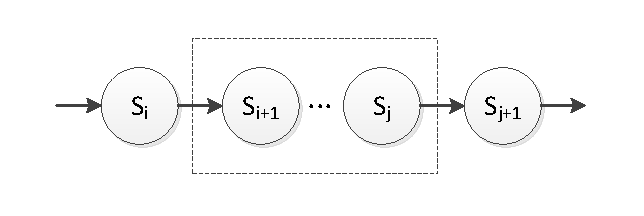
\includegraphics[width=3.5cm]{series.pdf}}
  \centerline{(a) 原子服务串行组合}
\end{minipage}
\hfill
\begin{minipage}{.48\linewidth}
  \centerline{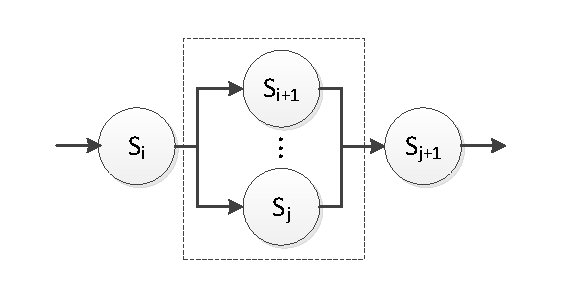
\includegraphics[width=3.5cm]{parallel.pdf}}
  \centerline{(b) 原子服务并行组合}{}
\end{minipage}
\vfill
\begin{minipage}{0.48\linewidth}
  \centerline{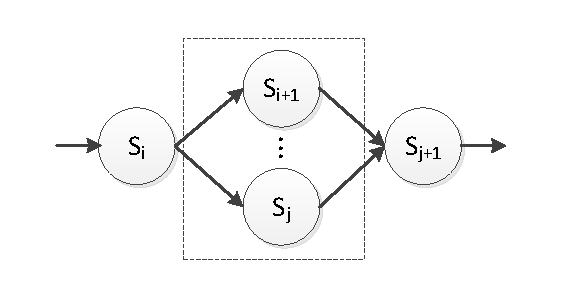
\includegraphics[width=3.5cm]{or.pdf}}
  \centerline{(c) 原子服务的选择}
\end{minipage}
\hfill
\begin{minipage}{0.48\linewidth}
  \centerline{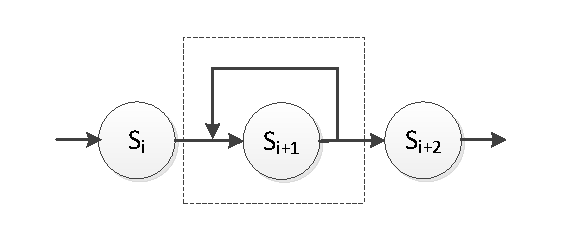
\includegraphics[width=3.5cm]{circle.pdf}}
  \centerline{(d) 原子服务的循环}
\end{minipage}
%\end{tabular}
\scriptsize\caption{服务组合的四种基本方式}
\label{fig:service_combine}
\end{figure}


\begin{figure}
\centering
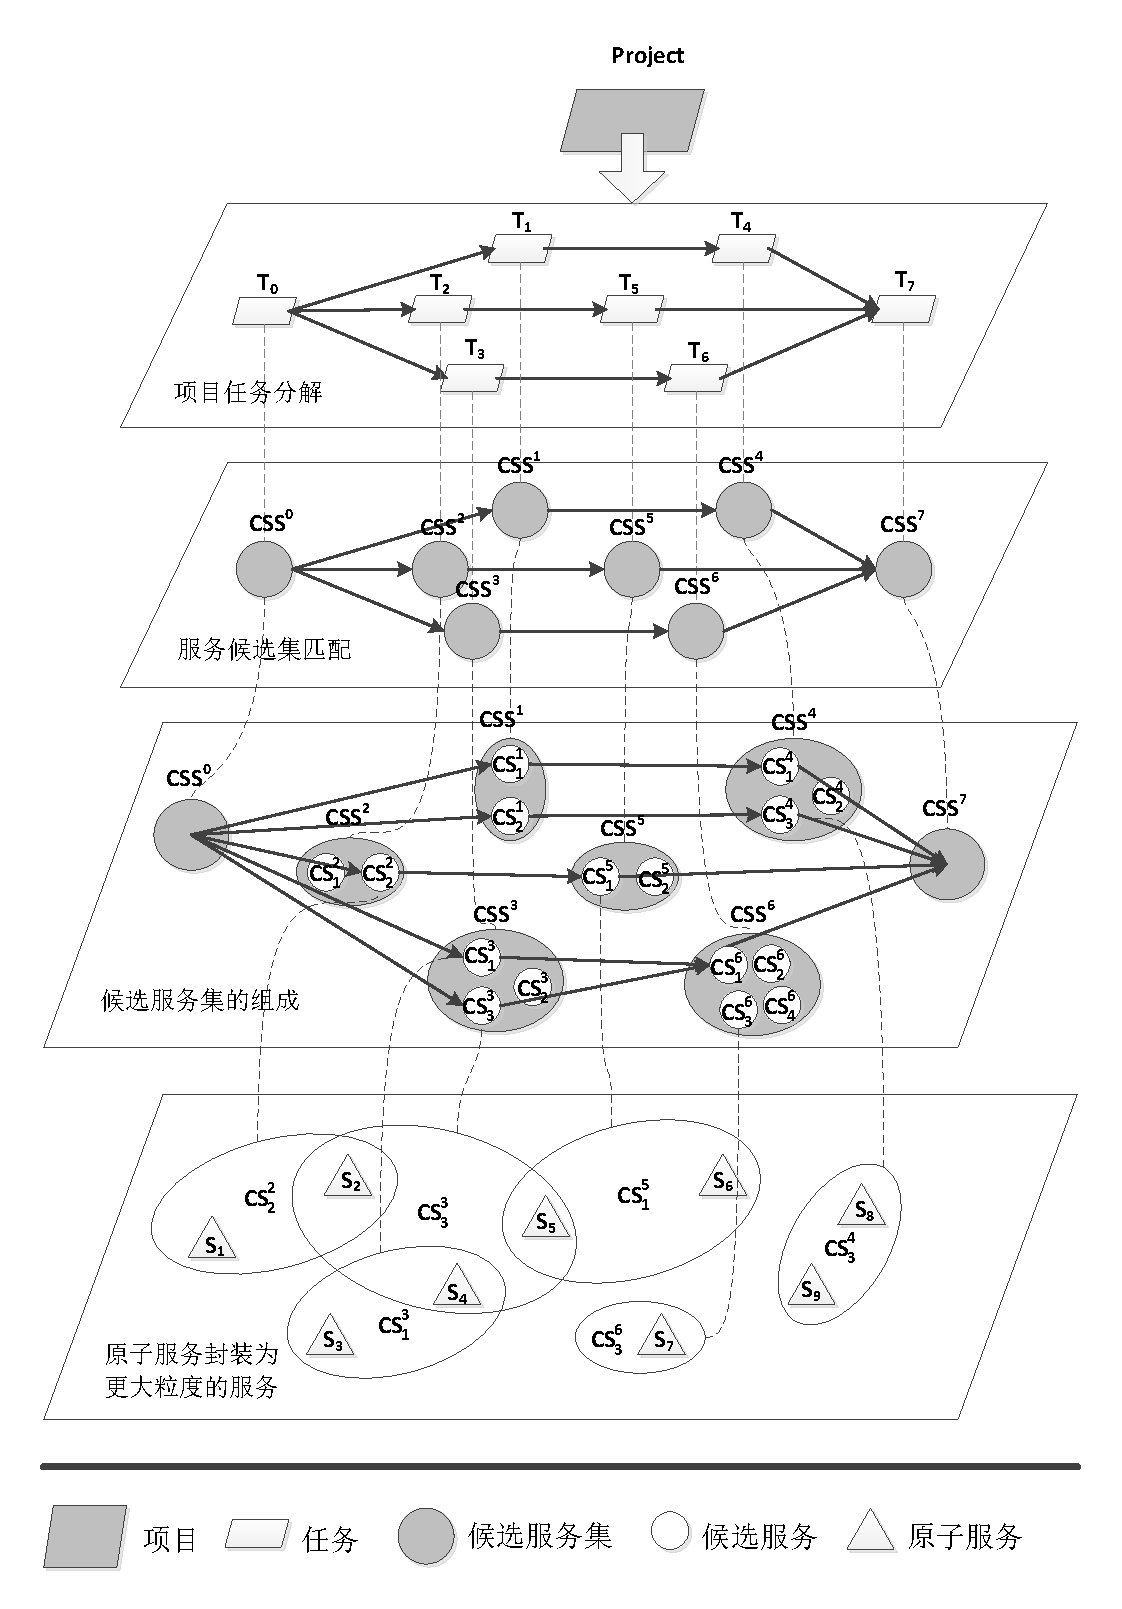
\includegraphics[width=.45\textwidth]{relation.pdf}
% \captionsetup{font=scriptsize}
\caption{云制造环境下服务组合优化实现方法}
\label{fig:relation}
\end{figure}

对于一个发布到云制造平台上的项目,云平台需要根据项目发布方所提出的要求(如项目的QoS属性的要求),为其匹配相应的服务并安排制造生产。其具体步骤如\cref{fig:relation}所示,需要经过项目任务分解、服务发现与匹配、服务组合优化、项目执行反馈这四个步骤。

(1)任务分解:一个发布到云平台上的项目$P$,平台根据其功能属性以及QoS属性,将其分解为较为合适的一个项目任务流程,任务集$T = \{T_0, T_1, \dots, T_n, T_{n + 1}\}$。其中,$n$为分解得到的任务数目,$T_0$和$T_{n + 1}$为虚拟任务,分别代表项目任务的起始和结束节点。

(2)服务匹配:根据分解得到的任一项目任务$T_j$的QoS属性,为其匹配得到相应的候选服务,形成候选服务集$CSS^j = \{CS_1^j, CS_2^j, \dots, CS_{K_j}^j\}$。其中$CS_k^j$表示制造任务$T_j$对应的第$k$个候选服务,$K_j$表示项目任务$T_j$的候选服务数量。将所有候选服务按顺序排列,则\\$CSS = \{CSS^0, CSS^1, CSS^2, \dots, CSS^j, \dots, CSS^n, CSS^{n + 1} \} \\ \quad =   \{CS_1^0, CS_1^1, CS_2^1, \dots, CS_{K_1}^1, \dots, CS_1^n, CS_2^n, \dots, CS_{K_n}^n, CS_1^{n + 1}\}$。其中,$CSS^0$和$CSS^{n + 1}$为虚拟候选服务集,$CS_0$和$CS_{n + 1}$为虚拟候选服务。 为简化表达,候选服务集表示为$CSS = \{CS_0, CS_1, CS_2, \dots, CS_K, CS_{K + 1}\}$。其中,$CS_k$为按顺序排列后的第$k$个候选服务,$K$为候选服务总数。

(3)服务组合优化:云平台根据候选服务为其配置相应的原子服务,原子服务集$S = \{S_1, S_2, \dots, S_L\}$,其中,$S_l$表示集合中的第$l$个原子服务,$L$表示集合中原子服务的总数。由于同时一种原子服务可能可以用来组成不同的更大粒度的候选服务,候选服务之间可能存在约束关系,需要通过服务组合优化来达成更优的全局策略。

(4)项目执行反馈:由于项目在执行过程中,外部环境是不断变化的,因此对于项目执行情况需要进行实时检测与调整。

为便于问题建模,我们作如下假设:

(1)一个原子服务一旦组成一个候选服务就必须服务该候选服务对应的制造任务,直至该制造任务完成。即制造任务对其候选服务及候选服务中的原子服务都具有独占性。

(2)受限于资源约束,原子服务或候选服务具有数量限制。原子服务的数量$\bm{b} = \{b_1, b_2, \dots, b_L\}$,其中,$b_l$为第$l$种原子服务的数量。

(3)由于并不影响最后结果,候选服务可认为是由原子服务按一定比例组成的。候选服务与原子服务的关系矩阵可表示为:

\[ \bm{A} = \begin{bmatrix}
a_{01} & \dots & a_{0L} \\
a_{11} & \dots & a_{1L} \\
\vdots & \ddots & \vdots \\
a_{K1} & \dots & a_{KL} \\
a_{K + 1, 1} & \dots & a_{K + 1, L}
\end{bmatrix} \]
\\
其中,矩阵中第一行和最后一行都为0,$a_{kl}$表示构成候选服务$CS_k$所需的原子服务$S_l$个数量,$a_{kl}$为非负整数。

云制造服务组合问题可分解为两个相互协同的子问题:
(1)在候选服务集中选择候选服务;
(2)根据选定的候选服务,对项目任务进行安排调度。

在选定候选服务集中的候选服务后,令矩阵$\bm{A}$中的未被选中的候选服务所在的行向量均变为零向量,然后对项目任务进行安排调度。
此时,该问题可以建立概念模型和整数规划模型两种模型。

此问题的概念模型中,主要存在两类约束。一类是项目任务之间的时序约束,另一类是支持该项目的原子服务的总量约束。

(1)项目任务的时序约束指的是任务执行的先后顺序。在项目的执行过程中,当一个项目任务没有完成时,它的后继任务无法开始执行。

\begin{equation}
\label{eq:con_seq}
C_h \leqslant C_j - p_j, \quad j = 1,\dots,n+1, h\in \mathcal{T}_j
\end{equation}

\cref{eq:con_seq}中,$C_j$表示任务$T_j$的完工时间,$p_j$表示任务$T_j$的加工时间,$C_h$表示任务$T_j$的前置任务的完工时间,$\mathcal{T}_j$为项目$T_h$所在的集合。

(2)原子服务的总量约束指的是,在项目执行过程中的任一时刻,组成候选服务的原子服务数量不能超过云平台上的现有原子服务数量。

\begin{equation}
\label{eq:con_amo}
\bm{A}^T \cdot \left(\sum_{T_j\in\Gamma_1(t)}s_{j,1},\dots, \sum_{T_j\in\Gamma_K(t)}s_{j,K} \right) \leqslant \bm{b}, \quad CS_k \in CSS, t \geqslant 0
\end{equation}

\cref{eq:con_amo}中,$\bm{A}^T$表示关系矩阵$\bm{A}$的转置。$\Gamma_k(t)=\{T_j|T_j\in T,c_j=CS_k, C_j-p_j\leqslant t < C_j\}$,为在时刻$t$(其中$C_j-p_j\leqslant t < C_j$)时, 且在候选服务$CSS_k$上的项目任务集合,其中,$c_j$表示项目任务$T_j$所选择的候选服务。\cref{fig:explain}解释了集合$\Gamma_k(t)$的含义,比如在时刻$t_1$,$\Gamma_k(t)$包含$T_i$和$T_j$两个项目任务,而在时刻$t_2$,$\Gamma_k(t)$只包含$T_j$一个项目任务。$s_{jk}$表示项目任务$T_j$所需的候选服务$CS_k$的数量,其值为非负整数。

(3)制造期非负约束,指的是任一项目的制造期都不可能为负。

\begin{equation}
\label{eq:con_completion_time}
C_j \geqslant 0, \qquad  T_j \in T
\end{equation}

\begin{figure}
\centering
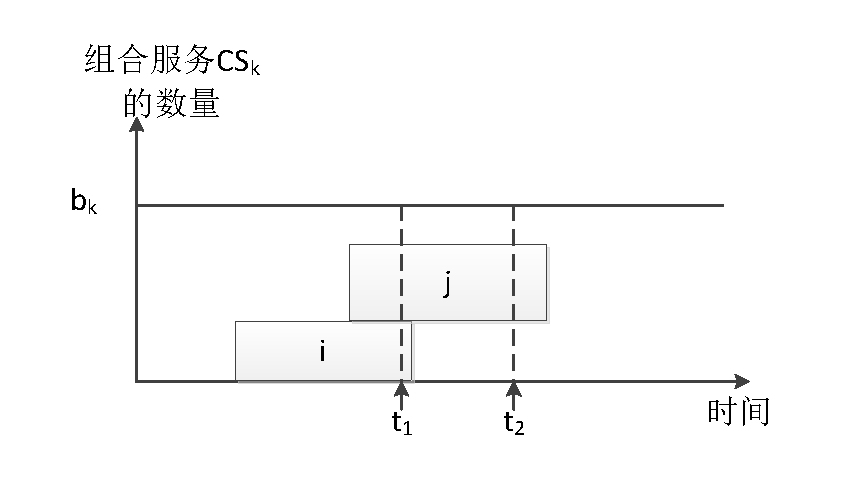
\includegraphics[width=.5\textwidth]{explain.pdf}
% \captionsetup{font=scriptsize}
\caption{\cref{eq:con_amo}的解释示意图}
\label{fig:explain}
\end{figure}

令$t$表示时间间隔$[t,t+1)$,决策变量$\xi_{jt}$用来决策任务$T_j$在时间$t$是否开始加工。$es_j$和$ls_j$分别表示任务$T_j$的最早可开始加工时间和最晚可开始加工时间。$\Gamma_k=\{T_j|T_j \in T, c_j = CS_k\}$表示在候选服务$CS_k$上的任务集合。其中,$\sigma(t,j)=\max(0,t-p_j+1)$,$T_{max}$为项目最迟完工时间。

(1)任一项目任务必须在其可执行的时间段内开始加工。

\begin{equation}
\label{eq:ip_dec_val}
\sum_{t = es_j}^{ls_j} \xi_{jt} = 1, \quad T_j \in T
\end{equation}

(2)项目任务的时序约束

\begin{equation}
\label{eq:ip_seq}
\sum_{t=es_h}^{ls_h} t\cdot\xi_{ht} \leqslant \sum_{t=es_j}^{ls_j} t\cdot\xi_{jt} - p_j, \quad  j = 1,\dots,n+1, h\in \mathcal{T}_j
\end{equation}

\cref{eq:ip_seq}中,$es_h$和$ls_h$分别表示任务$T_j$的前置任务的最早可开始时间和最晚可开始时间,$\mathcal{T}_j$为项目$T_h$所在的集合。

(3)原子服务的总量约束。

\begin{equation}
\label{eq:ip_amo}
\bm{A}^T\cdot \left(\sum_{T_j\in \Gamma_1} s_{j1} \sum_{\tau=\sigma(t,j)}^t \xi_{jt}, \dots, \sum_{T_j\in \Gamma_K} s_{jk} \sum_{\tau=\sigma(t,j)}^t \xi_{jt}\right) \leqslant \bm{b}, \quad  T_j \in T
\end{equation}

(4)相关参数的取值范围。

\begin{equation}
\label{eq:ip_dec_val}
\xi_{jt} \in \{0, 1\}, \quad  T_j\in T;\quad t = 0, \dots, T_{max}
\end{equation}

在项目调度中,以最小化制造期为优化目标的情况最为多见,这里也以项目的最小化制造期为目标函数。

(1)在概念模型中,概念模型的最小化制造期可表示为:

\begin{equation}
\label{eq:con_obj_func}
\text{Min} \qquad C_{n+1}
\end{equation}

(2)在整数规划模型中,整数规划模型的最小化制造期可表示为:

\begin{equation}
\label{eq:ip_obj_func}
\text{Min} \qquad \max\sum_{t=es_{n+1}}^{ls_{n+1}} t\cdot\xi_{it}
\end{equation}


\section{拟采用的求解方法}
\label{Sol}
本文简略地介绍了一下云制造环境下服务组合优化的问题。由于文中所述模型的复杂度巨大,在实际求解过程中常用的精确规划求解的数学方法难以应用。所以,在研究过程中采用进化算法作为主要的求解工具并且在求解算子中结合邻域搜索和规划求解的一些方法从而优化求解目标。

一些常用的求解器,比如CPLEX也被作为辅助求解工具用于求解本文所建立的模型。


\bibliographystyle{unsrt}
\bibliography{D:/biblib/science.bib}

\end{document}